\documentclass{book}
\usepackage[a4paper,top=2.5cm,bottom=2.5cm,left=2.5cm,right=2.5cm]{geometry}
\usepackage{makeidx}
\usepackage{natbib}
\usepackage{graphicx}
\usepackage{multicol}
\usepackage{float}
\usepackage{listings}
\usepackage{color}
\usepackage{ifthen}
\usepackage[table]{xcolor}
\usepackage{textcomp}
\usepackage{alltt}
\usepackage{ifpdf}
\ifpdf
\usepackage[pdftex,
            pagebackref=true,
            colorlinks=true,
            linkcolor=blue,
            unicode
           ]{hyperref}
\else
\usepackage[ps2pdf,
            pagebackref=true,
            colorlinks=true,
            linkcolor=blue,
            unicode
           ]{hyperref}
\usepackage{pspicture}
\fi
\usepackage[utf8]{inputenc}
\usepackage{mathptmx}
\usepackage[scaled=.90]{helvet}
\usepackage{courier}
\usepackage{sectsty}
\usepackage{amssymb}
\usepackage[titles]{tocloft}
\usepackage{doxygen}
\lstset{language=C++,inputencoding=utf8,basicstyle=\footnotesize,breaklines=true,breakatwhitespace=true,tabsize=8,numbers=left }
\makeindex
\setcounter{tocdepth}{3}
\renewcommand{\footrulewidth}{0.4pt}
\renewcommand{\familydefault}{\sfdefault}
\hfuzz=15pt
\setlength{\emergencystretch}{15pt}
\hbadness=750
\tolerance=750
\begin{document}
\hypersetup{pageanchor=false,citecolor=blue}
\begin{titlepage}
\vspace*{7cm}
\begin{center}
{\Large Lidar\-Eyeball \\[1ex]\large 0 }\\
\vspace*{1cm}
{\large Generated by Doxygen 1.8.3.1}\\
\vspace*{0.5cm}
{\small Tue Oct 8 2013 15:47:58}\\
\end{center}
\end{titlepage}
\clearemptydoublepage
\pagenumbering{roman}
\tableofcontents
\clearemptydoublepage
\pagenumbering{arabic}
\hypersetup{pageanchor=true,citecolor=blue}
\chapter{package Lidar\-Eyeball}
\label{index}\hypertarget{index}{}\begin{DoxyAuthor}{Authors}
J. Bregeon
\end{DoxyAuthor}
\hypertarget{index_intro}{}\section{Introduction}\label{index_intro}
Lidar\-Eyeball package to handle H\-E\-S\-S Lidar runs


\begin{DoxyItemize}
\item \hyperlink{index_pLidarRun}{Data analysis} \-: \hyperlink{pLidarRun_8py}{p\-Lidar\-Run.\-py} contains the p\-Lidar\-Run class to analyze Lidar data
\item \hyperlink{index_pLidarRunPlotter}{Analysis plotter} \-: \hyperlink{pLidarRunPlotter_8py}{p\-Lidar\-Run\-Plotter.\-py} contains the p\-Lidar\-Run\-Plotter calss to plot results from the Lidar analysis done with a p\-Lidar\-Run object
\item \hyperlink{index_tools}{Lidar analysis tool box} \-: \hyperlink{toolBox_8py}{tool\-Box.\-py}
\end{DoxyItemize}\hypertarget{index_pLidarRun}{}\section{Data analysis}\label{index_pLidarRun}
data analysis\hypertarget{index_pLidarRunPlotter}{}\section{Analysis plotter}\label{index_pLidarRunPlotter}
analysis plotter\hypertarget{index_tools}{}\section{Lidar analysis tool box}\label{index_tools}
\hyperlink{toolBox_8py}{tool\-Box.\-py} contains a set of functions to do stuff



 \begin{DoxyRefDesc}{Todo}
\item[\hyperlink{todo__todo000001}{Todo}]write documentation\end{DoxyRefDesc}

\chapter{Todo List}
\label{todo}
\hypertarget{todo}{}

\begin{DoxyRefList}
\item[\label{todo__todo000001}%
\hypertarget{todo__todo000001}{}%
page \hyperlink{index}{package Lidar\-Eyeball} ]write documentation
\end{DoxyRefList}
\chapter{Hierarchical Index}
\section{Class Hierarchy}
This inheritance list is sorted roughly, but not completely, alphabetically\-:\begin{DoxyCompactList}
\item object\begin{DoxyCompactList}
\item \contentsline{section}{p\-Lidar\-Run.\-p\-Lidar\-Run}{\pageref{classpLidarRun_1_1pLidarRun}}{}
\item \contentsline{section}{p\-Lidar\-Run\-Plotter.\-p\-Lidar\-Run\-Plotter}{\pageref{classpLidarRunPlotter_1_1pLidarRunPlotter}}{}
\end{DoxyCompactList}
\end{DoxyCompactList}

\chapter{Class Index}
\section{Class List}
Here are the classes, structs, unions and interfaces with brief descriptions\-:\begin{DoxyCompactList}
\item\contentsline{section}{\hyperlink{classpLidarRun_1_1pLidarRun}{p\-Lidar\-Run.\-p\-Lidar\-Run} \\*Class to manage a L\-I\-D\-A\-R run }{\pageref{classpLidarRun_1_1pLidarRun}}{}
\item\contentsline{section}{\hyperlink{classpLidarRunPlotter_1_1pLidarRunPlotter}{p\-Lidar\-Run\-Plotter.\-p\-Lidar\-Run\-Plotter} \\*Class to plot L\-I\-D\-A\-R run data }{\pageref{classpLidarRunPlotter_1_1pLidarRunPlotter}}{}
\end{DoxyCompactList}

\chapter{File Index}
\section{File List}
Here is a list of all documented files with brief descriptions\-:\begin{DoxyCompactList}
\item\contentsline{section}{/home/bregeon/\-C\-T\-A/\-Lidar/\-Lidar\-Eyeball/python/{\bfseries mainpage.\-h} }{\pageref{mainpage_8h}}{}
\item\contentsline{section}{/home/bregeon/\-C\-T\-A/\-Lidar/\-Lidar\-Eyeball/python/\hyperlink{pLidarRun_8py}{p\-Lidar\-Run.\-py} \\*The data analysis class }{\pageref{pLidarRun_8py}}{}
\item\contentsline{section}{/home/bregeon/\-C\-T\-A/\-Lidar/\-Lidar\-Eyeball/python/\hyperlink{pLidarRunPlotter_8py}{p\-Lidar\-Run\-Plotter.\-py} \\*The analysis plotter class }{\pageref{pLidarRunPlotter_8py}}{}
\item\contentsline{section}{/home/bregeon/\-C\-T\-A/\-Lidar/\-Lidar\-Eyeball/python/\hyperlink{toolBox_8py}{tool\-Box.\-py} \\*A set of Tools to be used in the Lidar\-Eyeball package }{\pageref{toolBox_8py}}{}
\end{DoxyCompactList}

\chapter{Class Documentation}
\hypertarget{classpLidarRun_1_1pLidarRun}{\section{p\-Lidar\-Run.\-p\-Lidar\-Run Class Reference}
\label{classpLidarRun_1_1pLidarRun}\index{p\-Lidar\-Run.\-p\-Lidar\-Run@{p\-Lidar\-Run.\-p\-Lidar\-Run}}
}


Class to manage a L\-I\-D\-A\-R run.  




Inheritance diagram for p\-Lidar\-Run.\-p\-Lidar\-Run\-:\nopagebreak
\begin{figure}[H]
\begin{center}
\leavevmode
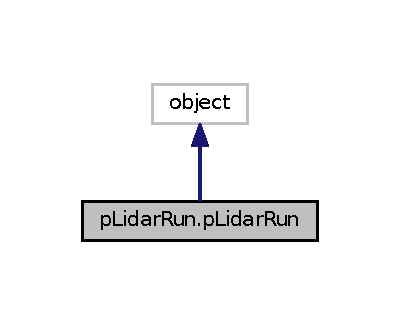
\includegraphics[width=192pt]{classpLidarRun_1_1pLidarRun__inherit__graph}
\end{center}
\end{figure}


Collaboration diagram for p\-Lidar\-Run.\-p\-Lidar\-Run\-:\nopagebreak
\begin{figure}[H]
\begin{center}
\leavevmode
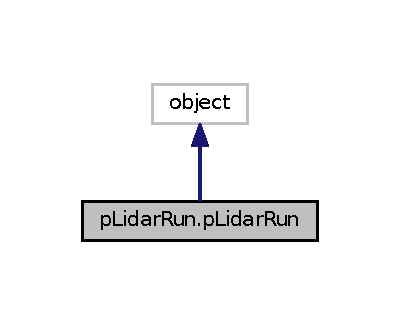
\includegraphics[width=192pt]{classpLidarRun_1_1pLidarRun__coll__graph}
\end{center}
\end{figure}
\subsection*{Public Member Functions}
\begin{DoxyCompactItemize}
\item 
def \hyperlink{classpLidarRun_1_1pLidarRun_a0d0e1c5a0637af2da72909d2e2deb3bb}{\-\_\-\-\_\-init\-\_\-\-\_\-}
\begin{DoxyCompactList}\small\item\em Constructor for a pulsar source. \end{DoxyCompactList}\item 
\hypertarget{classpLidarRun_1_1pLidarRun_a9a90df9e5b521ac30f30081d91c2b21f}{def {\bfseries read\-File}}\label{classpLidarRun_1_1pLidarRun_a9a90df9e5b521ac30f30081d91c2b21f}

\item 
def \hyperlink{classpLidarRun_1_1pLidarRun_a29d4e4ec14a225f956d7a553575f9e28}{process}
\begin{DoxyCompactList}\small\item\em Full processing including Klett inversion. \end{DoxyCompactList}\item 
def \hyperlink{classpLidarRun_1_1pLidarRun_a52586e96e8c5e346460d1dc19dd30911}{reduce}
\begin{DoxyCompactList}\small\item\em Subtract background and calculate power. \end{DoxyCompactList}\item 
\hypertarget{classpLidarRun_1_1pLidarRun_aabee77680300379f1769bdd19d326e55}{def {\bfseries ln\-Power}}\label{classpLidarRun_1_1pLidarRun_aabee77680300379f1769bdd19d326e55}

\item 
\hypertarget{classpLidarRun_1_1pLidarRun_a07b9a540eee11da513c902942e0278ab}{def {\bfseries simple\-Plot}}\label{classpLidarRun_1_1pLidarRun_a07b9a540eee11da513c902942e0278ab}

\item 
\hypertarget{classpLidarRun_1_1pLidarRun_a4cebf0f7e05b5a7939ccba93b65b65ff}{def {\bfseries bin\-Data}}\label{classpLidarRun_1_1pLidarRun_a4cebf0f7e05b5a7939ccba93b65b65ff}

\item 
def \hyperlink{classpLidarRun_1_1pLidarRun_a76e2ffb9b188fad04d51feb79acbd33c}{run\-\_\-\-Klett}
\begin{DoxyCompactList}\small\item\em Klett implementation P(r)=V(r)$\ast$r2 alpha(r)=P(r)/( P(r0)/alpha0 -\/ 2$\ast$sum\{r0,r\}\{P(h).dh\} ) \end{DoxyCompactList}\item 
def \hyperlink{classpLidarRun_1_1pLidarRun_a4844e3a98806f2351089092227ca997d}{Tau\-And\-Quality}
\begin{DoxyCompactList}\small\item\em Integrate Alpha to get absorption for the first h km From Tau4 in Piron et al Also use Tau4 to set run quality. \end{DoxyCompactList}\item 
def \hyperlink{classpLidarRun_1_1pLidarRun_a3253cb61ab67d3228ac146e0f843dfde}{calc\-Tau4}
\begin{DoxyCompactList}\small\item\em Integrate Alpha to get absorption for the first 4 km Tau4 in Piron et al. \end{DoxyCompactList}\item 
def \hyperlink{classpLidarRun_1_1pLidarRun_a9e852c0c83146f992308a9e903212cd7}{calc\-Transmission}
\begin{DoxyCompactList}\small\item\em Integrate Alpha to get absorption for the first 4 km Tau4 in Piron et al. \end{DoxyCompactList}\item 
def \hyperlink{classpLidarRun_1_1pLidarRun_ad2bfe11b5f2aef237a0bf6c937aed23f}{dump\-To\-Dict}
\begin{DoxyCompactList}\small\item\em Return a string for a dictionnary. \end{DoxyCompactList}\end{DoxyCompactItemize}
\subsection*{Public Attributes}
\begin{DoxyCompactItemize}
\item 
\hypertarget{classpLidarRun_1_1pLidarRun_ad8b058e3bda74e52a3d8d8598897ab87}{{\bfseries File\-Name}}\label{classpLidarRun_1_1pLidarRun_ad8b058e3bda74e52a3d8d8598897ab87}

\item 
\hypertarget{classpLidarRun_1_1pLidarRun_a78928c5e23b2aceb8150fd373d3786b0}{{\bfseries N\-Bins}}\label{classpLidarRun_1_1pLidarRun_a78928c5e23b2aceb8150fd373d3786b0}

\item 
\hypertarget{classpLidarRun_1_1pLidarRun_afbd07169ff6b311eed9b3864bca47049}{{\bfseries Run\-Number}}\label{classpLidarRun_1_1pLidarRun_afbd07169ff6b311eed9b3864bca47049}

\item 
\hypertarget{classpLidarRun_1_1pLidarRun_a48b227392af9892b7a47bc9df64b7d09}{{\bfseries Date\-Time}}\label{classpLidarRun_1_1pLidarRun_a48b227392af9892b7a47bc9df64b7d09}

\item 
\hypertarget{classpLidarRun_1_1pLidarRun_a64ab6c7fc15a0fcdfa89d2a3733fcdb9}{{\bfseries N\-Points}}\label{classpLidarRun_1_1pLidarRun_a64ab6c7fc15a0fcdfa89d2a3733fcdb9}

\item 
\hypertarget{classpLidarRun_1_1pLidarRun_ae2fe817bf22d99837c090b39a3e109ff}{{\bfseries Raw\-Data}}\label{classpLidarRun_1_1pLidarRun_ae2fe817bf22d99837c090b39a3e109ff}

\item 
\hypertarget{classpLidarRun_1_1pLidarRun_a8ed7352f80b39148f5792f68f8bf899c}{{\bfseries Raw\-Altitude}}\label{classpLidarRun_1_1pLidarRun_a8ed7352f80b39148f5792f68f8bf899c}

\item 
\hypertarget{classpLidarRun_1_1pLidarRun_a0c77a5c90517497c9354272425fc72a3}{{\bfseries Raw\-W\-L1}}\label{classpLidarRun_1_1pLidarRun_a0c77a5c90517497c9354272425fc72a3}

\item 
\hypertarget{classpLidarRun_1_1pLidarRun_a51ee3c53c62e948d14feddd1bcf99c9b}{{\bfseries Raw\-W\-L2}}\label{classpLidarRun_1_1pLidarRun_a51ee3c53c62e948d14feddd1bcf99c9b}

\item 
\hypertarget{classpLidarRun_1_1pLidarRun_aaa8178d2352f9364ded6f92d76f01163}{{\bfseries Alt\-Min}}\label{classpLidarRun_1_1pLidarRun_aaa8178d2352f9364ded6f92d76f01163}

\item 
\hypertarget{classpLidarRun_1_1pLidarRun_a4768e761dd4057f4ea2ffca23bb8b26f}{{\bfseries Alt\-Max}}\label{classpLidarRun_1_1pLidarRun_a4768e761dd4057f4ea2ffca23bb8b26f}

\item 
\hypertarget{classpLidarRun_1_1pLidarRun_ac942b30cb3fd5331c9add267f01561d2}{{\bfseries Bkg\-Min}}\label{classpLidarRun_1_1pLidarRun_ac942b30cb3fd5331c9add267f01561d2}

\item 
\hypertarget{classpLidarRun_1_1pLidarRun_af0d2dff114aebfaed7010248d9738b76}{{\bfseries Bkg\-Max}}\label{classpLidarRun_1_1pLidarRun_af0d2dff114aebfaed7010248d9738b76}

\item 
\hypertarget{classpLidarRun_1_1pLidarRun_ab844528398d99dd5e3a0f4f8b6dfb3fe}{{\bfseries Bkg\-Min\-Index}}\label{classpLidarRun_1_1pLidarRun_ab844528398d99dd5e3a0f4f8b6dfb3fe}

\item 
\hypertarget{classpLidarRun_1_1pLidarRun_ac528cb50b3535bf2bc7ee18d392e41c7}{{\bfseries Bkg\-Max\-Index}}\label{classpLidarRun_1_1pLidarRun_ac528cb50b3535bf2bc7ee18d392e41c7}

\item 
\hypertarget{classpLidarRun_1_1pLidarRun_a5c858b0626dec9bbca91e7d06196567e}{{\bfseries Alt\-Min\-Index}}\label{classpLidarRun_1_1pLidarRun_a5c858b0626dec9bbca91e7d06196567e}

\item 
\hypertarget{classpLidarRun_1_1pLidarRun_aebb0c352b2afa2838fbf08ccd86d34af}{{\bfseries Alt\-Max\-Index}}\label{classpLidarRun_1_1pLidarRun_aebb0c352b2afa2838fbf08ccd86d34af}

\item 
\hypertarget{classpLidarRun_1_1pLidarRun_a6543d548b23fbf1ed83843427172d0ef}{{\bfseries Bkg\-W\-L1}}\label{classpLidarRun_1_1pLidarRun_a6543d548b23fbf1ed83843427172d0ef}

\item 
\hypertarget{classpLidarRun_1_1pLidarRun_a033ba33e01d5cd5e2771b84bbd00f615}{{\bfseries Bkg\-W\-L2}}\label{classpLidarRun_1_1pLidarRun_a033ba33e01d5cd5e2771b84bbd00f615}

\item 
\hypertarget{classpLidarRun_1_1pLidarRun_ac86b50259771fa720936b9ec87aa6209}{{\bfseries W\-L1}}\label{classpLidarRun_1_1pLidarRun_ac86b50259771fa720936b9ec87aa6209}

\item 
\hypertarget{classpLidarRun_1_1pLidarRun_ac7fd8d3129b93479d8fbbe32c55457d2}{{\bfseries W\-L2}}\label{classpLidarRun_1_1pLidarRun_ac7fd8d3129b93479d8fbbe32c55457d2}

\item 
\hypertarget{classpLidarRun_1_1pLidarRun_a84d68c07e5d54adbded2bb3308997dc1}{{\bfseries Alt}}\label{classpLidarRun_1_1pLidarRun_a84d68c07e5d54adbded2bb3308997dc1}

\item 
\hypertarget{classpLidarRun_1_1pLidarRun_a58ea830e9ff8281c57dae6485848ebd8}{{\bfseries P\-W1}}\label{classpLidarRun_1_1pLidarRun_a58ea830e9ff8281c57dae6485848ebd8}

\item 
\hypertarget{classpLidarRun_1_1pLidarRun_a64330b0ec1a65dbc3354f6aecf911014}{{\bfseries P\-W2}}\label{classpLidarRun_1_1pLidarRun_a64330b0ec1a65dbc3354f6aecf911014}

\item 
\hypertarget{classpLidarRun_1_1pLidarRun_a6a4c9982c4b5ed0558a3989e41f086f6}{{\bfseries N\-Data}}\label{classpLidarRun_1_1pLidarRun_a6a4c9982c4b5ed0558a3989e41f086f6}

\item 
\hypertarget{classpLidarRun_1_1pLidarRun_a80ad0577ccd2f6e27e448db1eb4383b7}{{\bfseries Ln\-P\-W1}}\label{classpLidarRun_1_1pLidarRun_a80ad0577ccd2f6e27e448db1eb4383b7}

\item 
\hypertarget{classpLidarRun_1_1pLidarRun_a516c15b369b32168aaf93328c7ac4a85}{{\bfseries Ln\-P\-W2}}\label{classpLidarRun_1_1pLidarRun_a516c15b369b32168aaf93328c7ac4a85}

\item 
\hypertarget{classpLidarRun_1_1pLidarRun_aac0b316f18e0c35357e83c0875395c26}{{\bfseries Bin\-Ln\-Alt\-Width}}\label{classpLidarRun_1_1pLidarRun_aac0b316f18e0c35357e83c0875395c26}

\item 
\hypertarget{classpLidarRun_1_1pLidarRun_aeee4a352864e2fbbabf699904031458c}{{\bfseries Bins\-Alt}}\label{classpLidarRun_1_1pLidarRun_aeee4a352864e2fbbabf699904031458c}

\item 
\hypertarget{classpLidarRun_1_1pLidarRun_ad5ed34e9963844561b661fd35a195c4a}{{\bfseries Bins\-Alt\-Min}}\label{classpLidarRun_1_1pLidarRun_ad5ed34e9963844561b661fd35a195c4a}

\item 
\hypertarget{classpLidarRun_1_1pLidarRun_a58e31a52e1c5aee7ce05bdc357f7fd7d}{{\bfseries Bins\-Alt\-Max}}\label{classpLidarRun_1_1pLidarRun_a58e31a52e1c5aee7ce05bdc357f7fd7d}

\item 
\hypertarget{classpLidarRun_1_1pLidarRun_a6eac015144d813eb25a3370300af05e3}{{\bfseries Bins\-Alt\-Center}}\label{classpLidarRun_1_1pLidarRun_a6eac015144d813eb25a3370300af05e3}

\item 
\hypertarget{classpLidarRun_1_1pLidarRun_a5e7fb1031c654eea1b4ecadf81af191d}{{\bfseries Binned\-P\-W1}}\label{classpLidarRun_1_1pLidarRun_a5e7fb1031c654eea1b4ecadf81af191d}

\item 
\hypertarget{classpLidarRun_1_1pLidarRun_a5d8a059e8a4a6f1d22cf4838c6850e52}{{\bfseries Binned\-P\-W2}}\label{classpLidarRun_1_1pLidarRun_a5d8a059e8a4a6f1d22cf4838c6850e52}

\item 
\hypertarget{classpLidarRun_1_1pLidarRun_a52646321bb75f74cc2bc8817f093c2f4}{{\bfseries Binned\-Ln\-P\-W1}}\label{classpLidarRun_1_1pLidarRun_a52646321bb75f74cc2bc8817f093c2f4}

\item 
\hypertarget{classpLidarRun_1_1pLidarRun_a3af2c812d1169f92e7a999fc9aaab913}{{\bfseries Binned\-Ln\-P\-W2}}\label{classpLidarRun_1_1pLidarRun_a3af2c812d1169f92e7a999fc9aaab913}

\item 
\hypertarget{classpLidarRun_1_1pLidarRun_ab960b58c0901a9f7a205e9f1864c2797}{{\bfseries Binned\-Npoints}}\label{classpLidarRun_1_1pLidarRun_ab960b58c0901a9f7a205e9f1864c2797}

\item 
\hypertarget{classpLidarRun_1_1pLidarRun_af48dc918be044ab348a4bf7c5ad3d6b0}{{\bfseries Klett\-\_\-r0}}\label{classpLidarRun_1_1pLidarRun_af48dc918be044ab348a4bf7c5ad3d6b0}

\item 
\hypertarget{classpLidarRun_1_1pLidarRun_a6406cba149d3a47b1386bd5dfe13d5be}{{\bfseries Klett\-\_\-alpha0wl1}}\label{classpLidarRun_1_1pLidarRun_a6406cba149d3a47b1386bd5dfe13d5be}

\item 
\hypertarget{classpLidarRun_1_1pLidarRun_a107a53fdd4e65fdade3857868c68653c}{{\bfseries Klett\-\_\-alpha0wl2}}\label{classpLidarRun_1_1pLidarRun_a107a53fdd4e65fdade3857868c68653c}

\item 
\hypertarget{classpLidarRun_1_1pLidarRun_abcc6373b30622f57df0b721e3f24ba23}{{\bfseries Klett\-\_\-k}}\label{classpLidarRun_1_1pLidarRun_abcc6373b30622f57df0b721e3f24ba23}

\item 
\hypertarget{classpLidarRun_1_1pLidarRun_a9b9eff872e366999435f26b4e314c1c5}{{\bfseries Klett\-\_\-l}}\label{classpLidarRun_1_1pLidarRun_a9b9eff872e366999435f26b4e314c1c5}

\item 
\hypertarget{classpLidarRun_1_1pLidarRun_a9a60a5c850696db3d53b1e775aadbf6d}{{\bfseries Alpha\-N\-Bins}}\label{classpLidarRun_1_1pLidarRun_a9a60a5c850696db3d53b1e775aadbf6d}

\item 
\hypertarget{classpLidarRun_1_1pLidarRun_aec99c252ee7b458690e658afbd23a51e}{{\bfseries Binned\-Alpha\-P\-W1}}\label{classpLidarRun_1_1pLidarRun_aec99c252ee7b458690e658afbd23a51e}

\item 
\hypertarget{classpLidarRun_1_1pLidarRun_a14f87d0fdfaae0daca045378ceb86d27}{{\bfseries Binned\-Alpha\-P\-W2}}\label{classpLidarRun_1_1pLidarRun_a14f87d0fdfaae0daca045378ceb86d27}

\item 
\hypertarget{classpLidarRun_1_1pLidarRun_a077f848881c9617f86fe4466af50377a}{{\bfseries Tau4\-W\-L1}}\label{classpLidarRun_1_1pLidarRun_a077f848881c9617f86fe4466af50377a}

\item 
\hypertarget{classpLidarRun_1_1pLidarRun_aa8675a45076f3b8ebc2477efb570b528}{{\bfseries Tau4\-W\-L2}}\label{classpLidarRun_1_1pLidarRun_aa8675a45076f3b8ebc2477efb570b528}

\item 
\hypertarget{classpLidarRun_1_1pLidarRun_a91cc28fc9ffd680b5fc47e3fe6d29894}{{\bfseries Is\-Good}}\label{classpLidarRun_1_1pLidarRun_a91cc28fc9ffd680b5fc47e3fe6d29894}

\end{DoxyCompactItemize}


\subsection{Detailed Description}
Class to manage a L\-I\-D\-A\-R run. 

\subsection{Constructor \& Destructor Documentation}
\hypertarget{classpLidarRun_1_1pLidarRun_a0d0e1c5a0637af2da72909d2e2deb3bb}{\index{p\-Lidar\-Run\-::p\-Lidar\-Run@{p\-Lidar\-Run\-::p\-Lidar\-Run}!\-\_\-\-\_\-init\-\_\-\-\_\-@{\-\_\-\-\_\-init\-\_\-\-\_\-}}
\index{\-\_\-\-\_\-init\-\_\-\-\_\-@{\-\_\-\-\_\-init\-\_\-\-\_\-}!pLidarRun::pLidarRun@{p\-Lidar\-Run\-::p\-Lidar\-Run}}
\subsubsection[{\-\_\-\-\_\-init\-\_\-\-\_\-}]{\setlength{\rightskip}{0pt plus 5cm}def p\-Lidar\-Run.\-p\-Lidar\-Run.\-\_\-\-\_\-init\-\_\-\-\_\- (
\begin{DoxyParamCaption}
\item[{}]{self, }
\item[{}]{filename, }
\item[{}]{process = {\ttfamily True}, }
\item[{}]{n\-Bins = {\ttfamily 100}}
\end{DoxyParamCaption}
)}}\label{classpLidarRun_1_1pLidarRun_a0d0e1c5a0637af2da72909d2e2deb3bb}


Constructor for a pulsar source. 


\begin{DoxyParams}{Parameters}
{\em self} & the object instance \\
\hline
{\em filename} & a text file name with Lidar data \\
\hline
\end{DoxyParams}


\subsection{Member Function Documentation}
\hypertarget{classpLidarRun_1_1pLidarRun_a3253cb61ab67d3228ac146e0f843dfde}{\index{p\-Lidar\-Run\-::p\-Lidar\-Run@{p\-Lidar\-Run\-::p\-Lidar\-Run}!calc\-Tau4@{calc\-Tau4}}
\index{calc\-Tau4@{calc\-Tau4}!pLidarRun::pLidarRun@{p\-Lidar\-Run\-::p\-Lidar\-Run}}
\subsubsection[{calc\-Tau4}]{\setlength{\rightskip}{0pt plus 5cm}def p\-Lidar\-Run.\-p\-Lidar\-Run.\-calc\-Tau4 (
\begin{DoxyParamCaption}
\item[{}]{self}
\end{DoxyParamCaption}
)}}\label{classpLidarRun_1_1pLidarRun_a3253cb61ab67d3228ac146e0f843dfde}


Integrate Alpha to get absorption for the first 4 km Tau4 in Piron et al. 


\begin{DoxyParams}{Parameters}
{\em self} & the object instance \\
\hline
\end{DoxyParams}
\hypertarget{classpLidarRun_1_1pLidarRun_a9e852c0c83146f992308a9e903212cd7}{\index{p\-Lidar\-Run\-::p\-Lidar\-Run@{p\-Lidar\-Run\-::p\-Lidar\-Run}!calc\-Transmission@{calc\-Transmission}}
\index{calc\-Transmission@{calc\-Transmission}!pLidarRun::pLidarRun@{p\-Lidar\-Run\-::p\-Lidar\-Run}}
\subsubsection[{calc\-Transmission}]{\setlength{\rightskip}{0pt plus 5cm}def p\-Lidar\-Run.\-p\-Lidar\-Run.\-calc\-Transmission (
\begin{DoxyParamCaption}
\item[{}]{self, }
\item[{}]{h = {\ttfamily 4}}
\end{DoxyParamCaption}
)}}\label{classpLidarRun_1_1pLidarRun_a9e852c0c83146f992308a9e903212cd7}


Integrate Alpha to get absorption for the first 4 km Tau4 in Piron et al. 


\begin{DoxyParams}{Parameters}
{\em self} & the object instance \\
\hline
{\em h} & maximum altitude for intergration \\
\hline
\end{DoxyParams}
\hypertarget{classpLidarRun_1_1pLidarRun_ad2bfe11b5f2aef237a0bf6c937aed23f}{\index{p\-Lidar\-Run\-::p\-Lidar\-Run@{p\-Lidar\-Run\-::p\-Lidar\-Run}!dump\-To\-Dict@{dump\-To\-Dict}}
\index{dump\-To\-Dict@{dump\-To\-Dict}!pLidarRun::pLidarRun@{p\-Lidar\-Run\-::p\-Lidar\-Run}}
\subsubsection[{dump\-To\-Dict}]{\setlength{\rightskip}{0pt plus 5cm}def p\-Lidar\-Run.\-p\-Lidar\-Run.\-dump\-To\-Dict (
\begin{DoxyParamCaption}
\item[{}]{self}
\end{DoxyParamCaption}
)}}\label{classpLidarRun_1_1pLidarRun_ad2bfe11b5f2aef237a0bf6c937aed23f}


Return a string for a dictionnary. 


\begin{DoxyParams}{Parameters}
{\em self} & the object instance \\
\hline
\end{DoxyParams}
\hypertarget{classpLidarRun_1_1pLidarRun_a29d4e4ec14a225f956d7a553575f9e28}{\index{p\-Lidar\-Run\-::p\-Lidar\-Run@{p\-Lidar\-Run\-::p\-Lidar\-Run}!process@{process}}
\index{process@{process}!pLidarRun::pLidarRun@{p\-Lidar\-Run\-::p\-Lidar\-Run}}
\subsubsection[{process}]{\setlength{\rightskip}{0pt plus 5cm}def p\-Lidar\-Run.\-p\-Lidar\-Run.\-process (
\begin{DoxyParamCaption}
\item[{}]{self, }
\item[{}]{n\-Bins}
\end{DoxyParamCaption}
)}}\label{classpLidarRun_1_1pLidarRun_a29d4e4ec14a225f956d7a553575f9e28}


Full processing including Klett inversion. 


\begin{DoxyParams}{Parameters}
{\em self} & the object instance \\
\hline
{\em n\-Bins} & number of bins to use for calculations \\
\hline
\end{DoxyParams}
\hypertarget{classpLidarRun_1_1pLidarRun_a52586e96e8c5e346460d1dc19dd30911}{\index{p\-Lidar\-Run\-::p\-Lidar\-Run@{p\-Lidar\-Run\-::p\-Lidar\-Run}!reduce@{reduce}}
\index{reduce@{reduce}!pLidarRun::pLidarRun@{p\-Lidar\-Run\-::p\-Lidar\-Run}}
\subsubsection[{reduce}]{\setlength{\rightskip}{0pt plus 5cm}def p\-Lidar\-Run.\-p\-Lidar\-Run.\-reduce (
\begin{DoxyParamCaption}
\item[{}]{self, }
\item[{}]{altmin = {\ttfamily 0.800}, }
\item[{}]{altmax = {\ttfamily 10.}, }
\item[{}]{bkgmin = {\ttfamily 20.}, }
\item[{}]{bkgmax = {\ttfamily 25.}}
\end{DoxyParamCaption}
)}}\label{classpLidarRun_1_1pLidarRun_a52586e96e8c5e346460d1dc19dd30911}


Subtract background and calculate power. 


\begin{DoxyParams}{Parameters}
{\em self} & the object instance \\
\hline
{\em altmin} & minimum altitude to consider for signal \\
\hline
{\em altmax} & maximum altitute to consider for signal \\
\hline
{\em bkgmin} & minimum altitude to consider for background estimation \\
\hline
{\em bkgmax} & maximum altitute to consider for background estimation \\
\hline
\end{DoxyParams}
\hypertarget{classpLidarRun_1_1pLidarRun_a76e2ffb9b188fad04d51feb79acbd33c}{\index{p\-Lidar\-Run\-::p\-Lidar\-Run@{p\-Lidar\-Run\-::p\-Lidar\-Run}!run\-\_\-\-Klett@{run\-\_\-\-Klett}}
\index{run\-\_\-\-Klett@{run\-\_\-\-Klett}!pLidarRun::pLidarRun@{p\-Lidar\-Run\-::p\-Lidar\-Run}}
\subsubsection[{run\-\_\-\-Klett}]{\setlength{\rightskip}{0pt plus 5cm}def p\-Lidar\-Run.\-p\-Lidar\-Run.\-run\-\_\-\-Klett (
\begin{DoxyParamCaption}
\item[{}]{self, }
\item[{}]{r0 = {\ttfamily 10}, }
\item[{}]{alpha0wl1 = {\ttfamily 0.0038}, }
\item[{}]{alpha0wl2 = {\ttfamily 0.018}, }
\item[{}]{k = {\ttfamily 1}, }
\item[{}]{l = {\ttfamily 1}}
\end{DoxyParamCaption}
)}}\label{classpLidarRun_1_1pLidarRun_a76e2ffb9b188fad04d51feb79acbd33c}


Klett implementation P(r)=V(r)$\ast$r2 alpha(r)=P(r)/( P(r0)/alpha0 -\/ 2$\ast$sum\{r0,r\}\{P(h).dh\} ) 


\begin{DoxyParams}{Parameters}
{\em self} & the object instance \\
\hline
{\em r0} & reference altitude \\
\hline
{\em alpha0wl1} & alpha0 for wavelength 1 \\
\hline
{\em alpha0wl2} & alpha0 for wavelength 2 \\
\hline
{\em k} & as in beta=l$\ast$alpha$^\wedge$k \\
\hline
{\em l} & as in beta=l$\ast$alpha$^\wedge$k \\
\hline
\end{DoxyParams}
\hypertarget{classpLidarRun_1_1pLidarRun_a4844e3a98806f2351089092227ca997d}{\index{p\-Lidar\-Run\-::p\-Lidar\-Run@{p\-Lidar\-Run\-::p\-Lidar\-Run}!Tau\-And\-Quality@{Tau\-And\-Quality}}
\index{Tau\-And\-Quality@{Tau\-And\-Quality}!pLidarRun::pLidarRun@{p\-Lidar\-Run\-::p\-Lidar\-Run}}
\subsubsection[{Tau\-And\-Quality}]{\setlength{\rightskip}{0pt plus 5cm}def p\-Lidar\-Run.\-p\-Lidar\-Run.\-Tau\-And\-Quality (
\begin{DoxyParamCaption}
\item[{}]{self, }
\item[{}]{h = {\ttfamily 4}}
\end{DoxyParamCaption}
)}}\label{classpLidarRun_1_1pLidarRun_a4844e3a98806f2351089092227ca997d}


Integrate Alpha to get absorption for the first h km From Tau4 in Piron et al Also use Tau4 to set run quality. 


\begin{DoxyParams}{Parameters}
{\em self} & the object instance \\
\hline
{\em h} & maximum altitude for intergration \\
\hline
\end{DoxyParams}


The documentation for this class was generated from the following file\-:\begin{DoxyCompactItemize}
\item 
/home/bregeon/\-C\-T\-A/\-Lidar/\-Lidar\-Eyeball/python/\hyperlink{pLidarRun_8py}{p\-Lidar\-Run.\-py}\end{DoxyCompactItemize}

\hypertarget{classpLidarRunPlotter_1_1pLidarRunPlotter}{\section{p\-Lidar\-Run\-Plotter.\-p\-Lidar\-Run\-Plotter Class Reference}
\label{classpLidarRunPlotter_1_1pLidarRunPlotter}\index{p\-Lidar\-Run\-Plotter.\-p\-Lidar\-Run\-Plotter@{p\-Lidar\-Run\-Plotter.\-p\-Lidar\-Run\-Plotter}}
}


Class to plot L\-I\-D\-A\-R run data.  




Inheritance diagram for p\-Lidar\-Run\-Plotter.\-p\-Lidar\-Run\-Plotter\-:\nopagebreak
\begin{figure}[H]
\begin{center}
\leavevmode
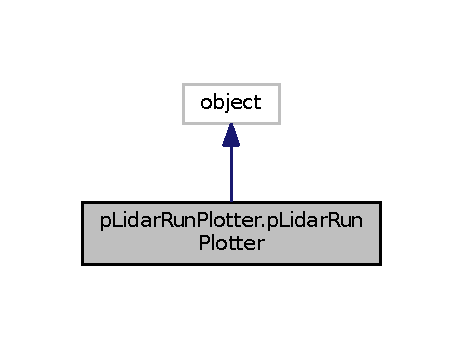
\includegraphics[width=222pt]{classpLidarRunPlotter_1_1pLidarRunPlotter__inherit__graph}
\end{center}
\end{figure}


Collaboration diagram for p\-Lidar\-Run\-Plotter.\-p\-Lidar\-Run\-Plotter\-:\nopagebreak
\begin{figure}[H]
\begin{center}
\leavevmode
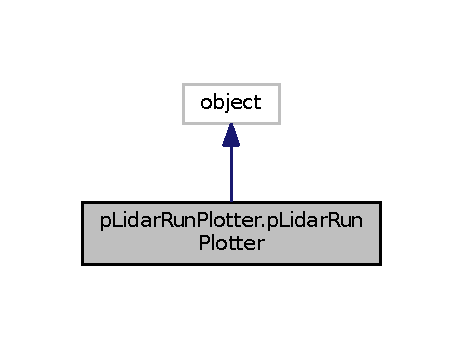
\includegraphics[width=222pt]{classpLidarRunPlotter_1_1pLidarRunPlotter__coll__graph}
\end{center}
\end{figure}
\subsection*{Public Member Functions}
\begin{DoxyCompactItemize}
\item 
def \hyperlink{classpLidarRunPlotter_1_1pLidarRunPlotter_aa7c1da9fb5a9a40bd906bc5cfb7f2a05}{\-\_\-\-\_\-init\-\_\-\-\_\-}
\begin{DoxyCompactList}\small\item\em Constructor for a pulsar source. \end{DoxyCompactList}\item 
\hypertarget{classpLidarRunPlotter_1_1pLidarRunPlotter_a19b05276bf9a374852923bbddd7a8176}{def {\bfseries fill\-Raw\-Data}}\label{classpLidarRunPlotter_1_1pLidarRunPlotter_a19b05276bf9a374852923bbddd7a8176}

\item 
\hypertarget{classpLidarRunPlotter_1_1pLidarRunPlotter_add0c52ed8c1e7724cd13738c81f3497f}{def {\bfseries fill\-Reduced\-Data}}\label{classpLidarRunPlotter_1_1pLidarRunPlotter_add0c52ed8c1e7724cd13738c81f3497f}

\item 
\hypertarget{classpLidarRunPlotter_1_1pLidarRunPlotter_a995d9a64e5f88b365cf02d96e8451e5b}{def {\bfseries fill\-Power\-Graphs}}\label{classpLidarRunPlotter_1_1pLidarRunPlotter_a995d9a64e5f88b365cf02d96e8451e5b}

\item 
\hypertarget{classpLidarRunPlotter_1_1pLidarRunPlotter_a7f781ecc2248c58547d10237940912ce}{def {\bfseries fill\-Ln\-Power\-Graphs}}\label{classpLidarRunPlotter_1_1pLidarRunPlotter_a7f781ecc2248c58547d10237940912ce}

\item 
\hypertarget{classpLidarRunPlotter_1_1pLidarRunPlotter_a396645d4e2ea2b850db1660501c99f16}{def {\bfseries fill\-Binned\-Power\-Graphs}}\label{classpLidarRunPlotter_1_1pLidarRunPlotter_a396645d4e2ea2b850db1660501c99f16}

\item 
\hypertarget{classpLidarRunPlotter_1_1pLidarRunPlotter_a80601d4a34a3fcd2b757d52c45480970}{def {\bfseries fill\-Binned\-Ln\-Power\-Graphs}}\label{classpLidarRunPlotter_1_1pLidarRunPlotter_a80601d4a34a3fcd2b757d52c45480970}

\item 
\hypertarget{classpLidarRunPlotter_1_1pLidarRunPlotter_a926b4db7270c22f58477073b0d057550}{def {\bfseries fill\-Klett\-Graphs}}\label{classpLidarRunPlotter_1_1pLidarRunPlotter_a926b4db7270c22f58477073b0d057550}

\item 
\hypertarget{classpLidarRunPlotter_1_1pLidarRunPlotter_afb309445317e864aa858c9fb01b1d176}{def {\bfseries fill\-All}}\label{classpLidarRunPlotter_1_1pLidarRunPlotter_afb309445317e864aa858c9fb01b1d176}

\item 
\hypertarget{classpLidarRunPlotter_1_1pLidarRunPlotter_ae18cb554204c049a6c105eaac70340a0}{def {\bfseries plot\-All}}\label{classpLidarRunPlotter_1_1pLidarRunPlotter_ae18cb554204c049a6c105eaac70340a0}

\item 
\hypertarget{classpLidarRunPlotter_1_1pLidarRunPlotter_aca76b2d77078d736d39db0c1fc8ac3d2}{def {\bfseries get\-Alpha}}\label{classpLidarRunPlotter_1_1pLidarRunPlotter_aca76b2d77078d736d39db0c1fc8ac3d2}

\item 
\hypertarget{classpLidarRunPlotter_1_1pLidarRunPlotter_aff08bc0a1ec8a35a086dbd9521190fdf}{def {\bfseries get\-Ln\-Power}}\label{classpLidarRunPlotter_1_1pLidarRunPlotter_aff08bc0a1ec8a35a086dbd9521190fdf}

\item 
\hypertarget{classpLidarRunPlotter_1_1pLidarRunPlotter_a9473b1c8c78ddde3ac3475d0795f8290}{def {\bfseries get\-Binned\-Ln\-Power}}\label{classpLidarRunPlotter_1_1pLidarRunPlotter_a9473b1c8c78ddde3ac3475d0795f8290}

\item 
\hypertarget{classpLidarRunPlotter_1_1pLidarRunPlotter_a350f08f3949c53e35992787db616a9cb}{def {\bfseries plot\-Both\-Power}}\label{classpLidarRunPlotter_1_1pLidarRunPlotter_a350f08f3949c53e35992787db616a9cb}

\item 
\hypertarget{classpLidarRunPlotter_1_1pLidarRunPlotter_ab0233b365dcedb6108fb0b9def78ab1c}{def {\bfseries plot\-Both\-Ln\-Power}}\label{classpLidarRunPlotter_1_1pLidarRunPlotter_ab0233b365dcedb6108fb0b9def78ab1c}

\item 
\hypertarget{classpLidarRunPlotter_1_1pLidarRunPlotter_ac7eb93dabb199c2c20ef912c4c0a6143}{def {\bfseries plot\-Both\-Alpha}}\label{classpLidarRunPlotter_1_1pLidarRunPlotter_ac7eb93dabb199c2c20ef912c4c0a6143}

\item 
\hypertarget{classpLidarRunPlotter_1_1pLidarRunPlotter_a42b9629690c61af80f6c84a344e81cd5}{def {\bfseries plot\-One\-Ln\-Power}}\label{classpLidarRunPlotter_1_1pLidarRunPlotter_a42b9629690c61af80f6c84a344e81cd5}

\item 
\hypertarget{classpLidarRunPlotter_1_1pLidarRunPlotter_a867a5d454e457a490b0910d6bf9097c4}{def {\bfseries plot\-One\-Alpha}}\label{classpLidarRunPlotter_1_1pLidarRunPlotter_a867a5d454e457a490b0910d6bf9097c4}

\end{DoxyCompactItemize}
\subsection*{Public Attributes}
\begin{DoxyCompactItemize}
\item 
\hypertarget{classpLidarRunPlotter_1_1pLidarRunPlotter_a84490f06a5ba103ebcf9adff82030b10}{{\bfseries Lidar\-Run}}\label{classpLidarRunPlotter_1_1pLidarRunPlotter_a84490f06a5ba103ebcf9adff82030b10}

\item 
\hypertarget{classpLidarRunPlotter_1_1pLidarRunPlotter_ab34b092bf026735a94435e4a6e651451}{{\bfseries g\-Raw\-W\-L1}}\label{classpLidarRunPlotter_1_1pLidarRunPlotter_ab34b092bf026735a94435e4a6e651451}

\item 
\hypertarget{classpLidarRunPlotter_1_1pLidarRunPlotter_a59d38246191814e284a4a1029932b9e1}{{\bfseries g\-Raw\-W\-L2}}\label{classpLidarRunPlotter_1_1pLidarRunPlotter_a59d38246191814e284a4a1029932b9e1}

\item 
\hypertarget{classpLidarRunPlotter_1_1pLidarRunPlotter_adb373be462908c517c17527baca9ea72}{{\bfseries g\-Reduced\-W\-L1}}\label{classpLidarRunPlotter_1_1pLidarRunPlotter_adb373be462908c517c17527baca9ea72}

\item 
\hypertarget{classpLidarRunPlotter_1_1pLidarRunPlotter_ab2d470dfafac14014f3f10b8ab365c51}{{\bfseries g\-Reduced\-W\-L2}}\label{classpLidarRunPlotter_1_1pLidarRunPlotter_ab2d470dfafac14014f3f10b8ab365c51}

\item 
\hypertarget{classpLidarRunPlotter_1_1pLidarRunPlotter_accba3ef56e755d76d7f29dd15b44978a}{{\bfseries g\-Power\-W\-L1}}\label{classpLidarRunPlotter_1_1pLidarRunPlotter_accba3ef56e755d76d7f29dd15b44978a}

\item 
\hypertarget{classpLidarRunPlotter_1_1pLidarRunPlotter_a35a1da734f75510a4d21bfa3f6bea9e2}{{\bfseries g\-Power\-W\-L2}}\label{classpLidarRunPlotter_1_1pLidarRunPlotter_a35a1da734f75510a4d21bfa3f6bea9e2}

\item 
\hypertarget{classpLidarRunPlotter_1_1pLidarRunPlotter_aefb871a46dd3144e959f06dea2d056e2}{{\bfseries g\-Ln\-Power\-W\-L1}}\label{classpLidarRunPlotter_1_1pLidarRunPlotter_aefb871a46dd3144e959f06dea2d056e2}

\item 
\hypertarget{classpLidarRunPlotter_1_1pLidarRunPlotter_a4cc6d55a17aed5fb1abf52e5d6e39063}{{\bfseries g\-Ln\-Power\-W\-L2}}\label{classpLidarRunPlotter_1_1pLidarRunPlotter_a4cc6d55a17aed5fb1abf52e5d6e39063}

\item 
\hypertarget{classpLidarRunPlotter_1_1pLidarRunPlotter_a6c7964162f85d014829db947cc1eb979}{{\bfseries g\-Binned\-Power\-W\-L1}}\label{classpLidarRunPlotter_1_1pLidarRunPlotter_a6c7964162f85d014829db947cc1eb979}

\item 
\hypertarget{classpLidarRunPlotter_1_1pLidarRunPlotter_abfe1ea57849659b039311f3c0528dace}{{\bfseries g\-Binned\-Power\-W\-L2}}\label{classpLidarRunPlotter_1_1pLidarRunPlotter_abfe1ea57849659b039311f3c0528dace}

\item 
\hypertarget{classpLidarRunPlotter_1_1pLidarRunPlotter_a298cda3f54b34deaa7152e88a2fdc099}{{\bfseries g\-Binned\-Ln\-Power\-W\-L1}}\label{classpLidarRunPlotter_1_1pLidarRunPlotter_a298cda3f54b34deaa7152e88a2fdc099}

\item 
\hypertarget{classpLidarRunPlotter_1_1pLidarRunPlotter_aa3ae00046ad6e037f9f7565c71ebd00c}{{\bfseries g\-Binned\-Ln\-Power\-W\-L2}}\label{classpLidarRunPlotter_1_1pLidarRunPlotter_aa3ae00046ad6e037f9f7565c71ebd00c}

\item 
\hypertarget{classpLidarRunPlotter_1_1pLidarRunPlotter_a1236faadf073e4388515ba67d30fe5ab}{{\bfseries g\-Binned\-Alpha\-P\-W1}}\label{classpLidarRunPlotter_1_1pLidarRunPlotter_a1236faadf073e4388515ba67d30fe5ab}

\item 
\hypertarget{classpLidarRunPlotter_1_1pLidarRunPlotter_a4fade797cfca91ffe02ebc27adcefdff}{{\bfseries g\-Binned\-Alpha\-P\-W2}}\label{classpLidarRunPlotter_1_1pLidarRunPlotter_a4fade797cfca91ffe02ebc27adcefdff}

\item 
\hypertarget{classpLidarRunPlotter_1_1pLidarRunPlotter_a149ca96344a76e4b6acb9e3d47d8aba2}{{\bfseries Main\-Canvas}}\label{classpLidarRunPlotter_1_1pLidarRunPlotter_a149ca96344a76e4b6acb9e3d47d8aba2}

\item 
\hypertarget{classpLidarRunPlotter_1_1pLidarRunPlotter_ac5a2c28427c7baaf20bf8a76a4b87f00}{{\bfseries P\-W\-Canvas}}\label{classpLidarRunPlotter_1_1pLidarRunPlotter_ac5a2c28427c7baaf20bf8a76a4b87f00}

\item 
\hypertarget{classpLidarRunPlotter_1_1pLidarRunPlotter_a33e0868ecda867b1f8f61dc6e200ea52}{{\bfseries Ln\-P\-W\-Canvas}}\label{classpLidarRunPlotter_1_1pLidarRunPlotter_a33e0868ecda867b1f8f61dc6e200ea52}

\item 
\hypertarget{classpLidarRunPlotter_1_1pLidarRunPlotter_a36fc6a7e619e15a076f95b9922ada894}{{\bfseries Alpha\-Canvas}}\label{classpLidarRunPlotter_1_1pLidarRunPlotter_a36fc6a7e619e15a076f95b9922ada894}

\item 
\hypertarget{classpLidarRunPlotter_1_1pLidarRunPlotter_a92effaf92aec84e7ff9016883f843f30}{{\bfseries g\-Alpha\-Canvas}}\label{classpLidarRunPlotter_1_1pLidarRunPlotter_a92effaf92aec84e7ff9016883f843f30}

\end{DoxyCompactItemize}


\subsection{Detailed Description}
Class to plot L\-I\-D\-A\-R run data. 

\subsection{Constructor \& Destructor Documentation}
\hypertarget{classpLidarRunPlotter_1_1pLidarRunPlotter_aa7c1da9fb5a9a40bd906bc5cfb7f2a05}{\index{p\-Lidar\-Run\-Plotter\-::p\-Lidar\-Run\-Plotter@{p\-Lidar\-Run\-Plotter\-::p\-Lidar\-Run\-Plotter}!\-\_\-\-\_\-init\-\_\-\-\_\-@{\-\_\-\-\_\-init\-\_\-\-\_\-}}
\index{\-\_\-\-\_\-init\-\_\-\-\_\-@{\-\_\-\-\_\-init\-\_\-\-\_\-}!pLidarRunPlotter::pLidarRunPlotter@{p\-Lidar\-Run\-Plotter\-::p\-Lidar\-Run\-Plotter}}
\subsubsection[{\-\_\-\-\_\-init\-\_\-\-\_\-}]{\setlength{\rightskip}{0pt plus 5cm}def p\-Lidar\-Run\-Plotter.\-p\-Lidar\-Run\-Plotter.\-\_\-\-\_\-init\-\_\-\-\_\- (
\begin{DoxyParamCaption}
\item[{}]{self, }
\item[{}]{lidar\-Run = {\ttfamily None}}
\end{DoxyParamCaption}
)}}\label{classpLidarRunPlotter_1_1pLidarRunPlotter_aa7c1da9fb5a9a40bd906bc5cfb7f2a05}


Constructor for a pulsar source. 


\begin{DoxyParams}{Parameters}
{\em self} & the object instance \\
\hline
{\em p\-Lidar\-Run} & a p\-Lidar\-Run object \\
\hline
\end{DoxyParams}


The documentation for this class was generated from the following file\-:\begin{DoxyCompactItemize}
\item 
/home/bregeon/\-C\-T\-A/\-Lidar/\-Lidar\-Eyeball/python/\hyperlink{pLidarRunPlotter_8py}{p\-Lidar\-Run\-Plotter.\-py}\end{DoxyCompactItemize}

\chapter{File Documentation}
\hypertarget{pLidarRun_8py}{\section{/home/bregeon/\-C\-T\-A/\-Lidar/\-Lidar\-Eyeball/python/p\-Lidar\-Run.py File Reference}
\label{pLidarRun_8py}\index{/home/bregeon/\-C\-T\-A/\-Lidar/\-Lidar\-Eyeball/python/p\-Lidar\-Run.\-py@{/home/bregeon/\-C\-T\-A/\-Lidar/\-Lidar\-Eyeball/python/p\-Lidar\-Run.\-py}}
}


The data analysis class.  


\subsection*{Classes}
\begin{DoxyCompactItemize}
\item 
class \hyperlink{classpLidarRun_1_1pLidarRun}{p\-Lidar\-Run.\-p\-Lidar\-Run}
\begin{DoxyCompactList}\small\item\em Class to manage a L\-I\-D\-A\-R run. \end{DoxyCompactList}\end{DoxyCompactItemize}
\subsection*{Variables}
\begin{DoxyCompactItemize}
\item 
\hypertarget{namespacepLidarRun_a25bf5fb44799a0ff8211f460e2566884}{string {\bfseries p\-Lidar\-Run.\-D\-A\-T\-A\-\_\-\-D\-I\-R} = '/home/bregeon/C\-T\-A/Lidar/alldata'}\label{namespacepLidarRun_a25bf5fb44799a0ff8211f460e2566884}

\item 
\hypertarget{namespacepLidarRun_a5fe8459835627ea3c7b60034f9d9fe19}{tuple {\bfseries p\-Lidar\-Run.\-r} = p\-Lidar\-Run(os.\-path.\-join(D\-A\-T\-A\-\_\-\-D\-I\-R,'run\-\_\-065160\-\_\-\-Lidar\-\_\-001.\-root.\-txt'), n\-Bins=100)}\label{namespacepLidarRun_a5fe8459835627ea3c7b60034f9d9fe19}

\end{DoxyCompactItemize}


\subsection{Detailed Description}
The data analysis class. 
\hypertarget{pLidarRunPlotter_8py}{\section{/home/bregeon/\-C\-T\-A/\-Lidar/\-Lidar\-Eyeball/python/p\-Lidar\-Run\-Plotter.py File Reference}
\label{pLidarRunPlotter_8py}\index{/home/bregeon/\-C\-T\-A/\-Lidar/\-Lidar\-Eyeball/python/p\-Lidar\-Run\-Plotter.\-py@{/home/bregeon/\-C\-T\-A/\-Lidar/\-Lidar\-Eyeball/python/p\-Lidar\-Run\-Plotter.\-py}}
}


The analysis plotter class.  


\subsection*{Classes}
\begin{DoxyCompactItemize}
\item 
class \hyperlink{classpLidarRunPlotter_1_1pLidarRunPlotter}{p\-Lidar\-Run\-Plotter.\-p\-Lidar\-Run\-Plotter}
\begin{DoxyCompactList}\small\item\em Class to plot L\-I\-D\-A\-R run data. \end{DoxyCompactList}\end{DoxyCompactItemize}
\subsection*{Variables}
\begin{DoxyCompactItemize}
\item 
\hypertarget{namespacepLidarRunPlotter_a244c031ca206e95ea322b9819ea954da}{tuple {\bfseries p\-Lidar\-Run\-Plotter.\-run} = \hyperlink{classpLidarRun_1_1pLidarRun}{p\-Lidar\-Run.\-p\-Lidar\-Run}('alldata/run\-\_\-069377\-\_\-\-Lidar\-\_\-001.\-root.\-txt',process=True, n\-Bins=100)}\label{namespacepLidarRunPlotter_a244c031ca206e95ea322b9819ea954da}

\item 
\hypertarget{namespacepLidarRunPlotter_a011e8d577375b45e4fa8e16a40b27625}{tuple {\bfseries p\-Lidar\-Run\-Plotter.\-plotter} = p\-Lidar\-Run\-Plotter(run)}\label{namespacepLidarRunPlotter_a011e8d577375b45e4fa8e16a40b27625}

\item 
\hypertarget{namespacepLidarRunPlotter_a5a644d39e3f07b52682e5c2bcac45d5f}{tuple {\bfseries p\-Lidar\-Run\-Plotter.\-c} = R\-O\-O\-T.\-T\-Canvas()}\label{namespacepLidarRunPlotter_a5a644d39e3f07b52682e5c2bcac45d5f}

\end{DoxyCompactItemize}


\subsection{Detailed Description}
The analysis plotter class. 
\hypertarget{toolBox_8py}{\section{/home/bregeon/\-C\-T\-A/\-Lidar/\-Lidar\-Eyeball/python/tool\-Box.py File Reference}
\label{toolBox_8py}\index{/home/bregeon/\-C\-T\-A/\-Lidar/\-Lidar\-Eyeball/python/tool\-Box.\-py@{/home/bregeon/\-C\-T\-A/\-Lidar/\-Lidar\-Eyeball/python/tool\-Box.\-py}}
}


A set of Tools to be used in the Lidar\-Eyeball package.  


\subsection*{Functions}
\begin{DoxyCompactItemize}
\item 
def {\bfseries tool\-Box.\-get\-Trans\-Prob}
\begin{DoxyCompactList}\small\item\em Simple estimate of the transmission probability and its variation given 2 Tau4. \end{DoxyCompactList}\item 
def {\bfseries tool\-Box.\-get\-Runs\-For\-Night}
\begin{DoxyCompactList}\small\item\em Get run numbers for a given night, using the run dictionnary L\-I\-D\-A\-R\-\_\-\-R\-U\-N\-\_\-\-D\-I\-C\-T. \end{DoxyCompactList}\item 
def {\bfseries tool\-Box.\-get\-Runs\-From\-To}
\begin{DoxyCompactList}\small\item\em Get run numbers for a given period, using the run dictionnary L\-I\-D\-A\-R\-\_\-\-R\-U\-N\-\_\-\-D\-I\-C\-T. \end{DoxyCompactList}\end{DoxyCompactItemize}


\subsection{Detailed Description}
A set of Tools to be used in the Lidar\-Eyeball package. 
\addcontentsline{toc}{part}{Index}
\printindex
\end{document}
